\documentclass[10pt, a4paper]{report}


\usepackage[left=15mm, top=20mm, right=15mm, bottom=20mm]{geometry}

\usepackage[utf8]{inputenc}
\usepackage[english,russian]{babel}
\usepackage{mflogo}
\usepackage{amsmath,amsfonts,amssymb}
\usepackage{xcolor}
\usepackage{graphicx}
\usepackage{cite}
\usepackage{multicol}


\usepackage{amsthm,amsmath}
\usepackage[shortlabels]{enumitem}
\usepackage{biblatex}

\renewcommand{\qedsymbol}{$\blacksquare$}



\renewcommand{\Im}{\mathop{\mathrm{Im}}\nolimits}
\renewcommand{\Re}{\mathop{\mathrm{Re}}\nolimits}
\renewcommand{\cot}{\mathop{\mathrm{ctg}}\nolimits}
\renewcommand{\sinh}{\mathop{\mathrm{sh}}\nolimits}
\renewcommand{\cosh}{\mathop{\mathrm{ch}}\nolimits}
\renewcommand{\arctan}{\mathop{\mathrm{arctg}}\nolimits}
\renewcommand{\tan}{\mathop{\mathrm{tg}}\nolimits}
\renewcommand{\tanh}{\mathop{\mathrm{th}}\nolimits}
\renewcommand{\sinh}{\mathop{\mathrm{sh}}\nolimits}
\renewcommand{\cosh}{\mathop{\mathrm{ch}}\nolimits}
\renewcommand{\coth}{\mathop{\mathrm{ctgh}}\nolimits}
\renewcommand{\log}{\ln}
\DeclareMathOperator{\lcm}{lcm}



\newcommand{\mychapter}[2]{
	\setcounter{chapter}{#1}
	\setcounter{section}{0}
	\chapter*{#2}
	\addcontentsline{toc}{chapter}{#2}
}

\setlength{\parskip}{0.5cm}

\graphicspath{{images/}}

\title{Оценка числа компонент графа итерации случайного отображения}
\author{Автор: Михалицын Пётр Константинович \\ Научный руководитель: Старший преподаватель кафедры "Компьютерная безопасность" \\ Миронкин Владимир Олегович}
\date{30 апреля 2018 г.}

\begin{document}
\maketitle
\tableofcontents

\mychapter{1}{Введение}

\mychapter{2}{Оценка числа компонент графа отображения}

\section{Случай любого случайного отображения}
Прежде чем начать поиск числа компонент графа случайного для начала определим как выглядит граф случайного отображения.

В первую очередь рассмотрим несколько примеров графов случайных отображений, чтобы приблизительно понять, с чем мы будем иметь дела и что считать.

\begin{figure}[h]
	\centering
	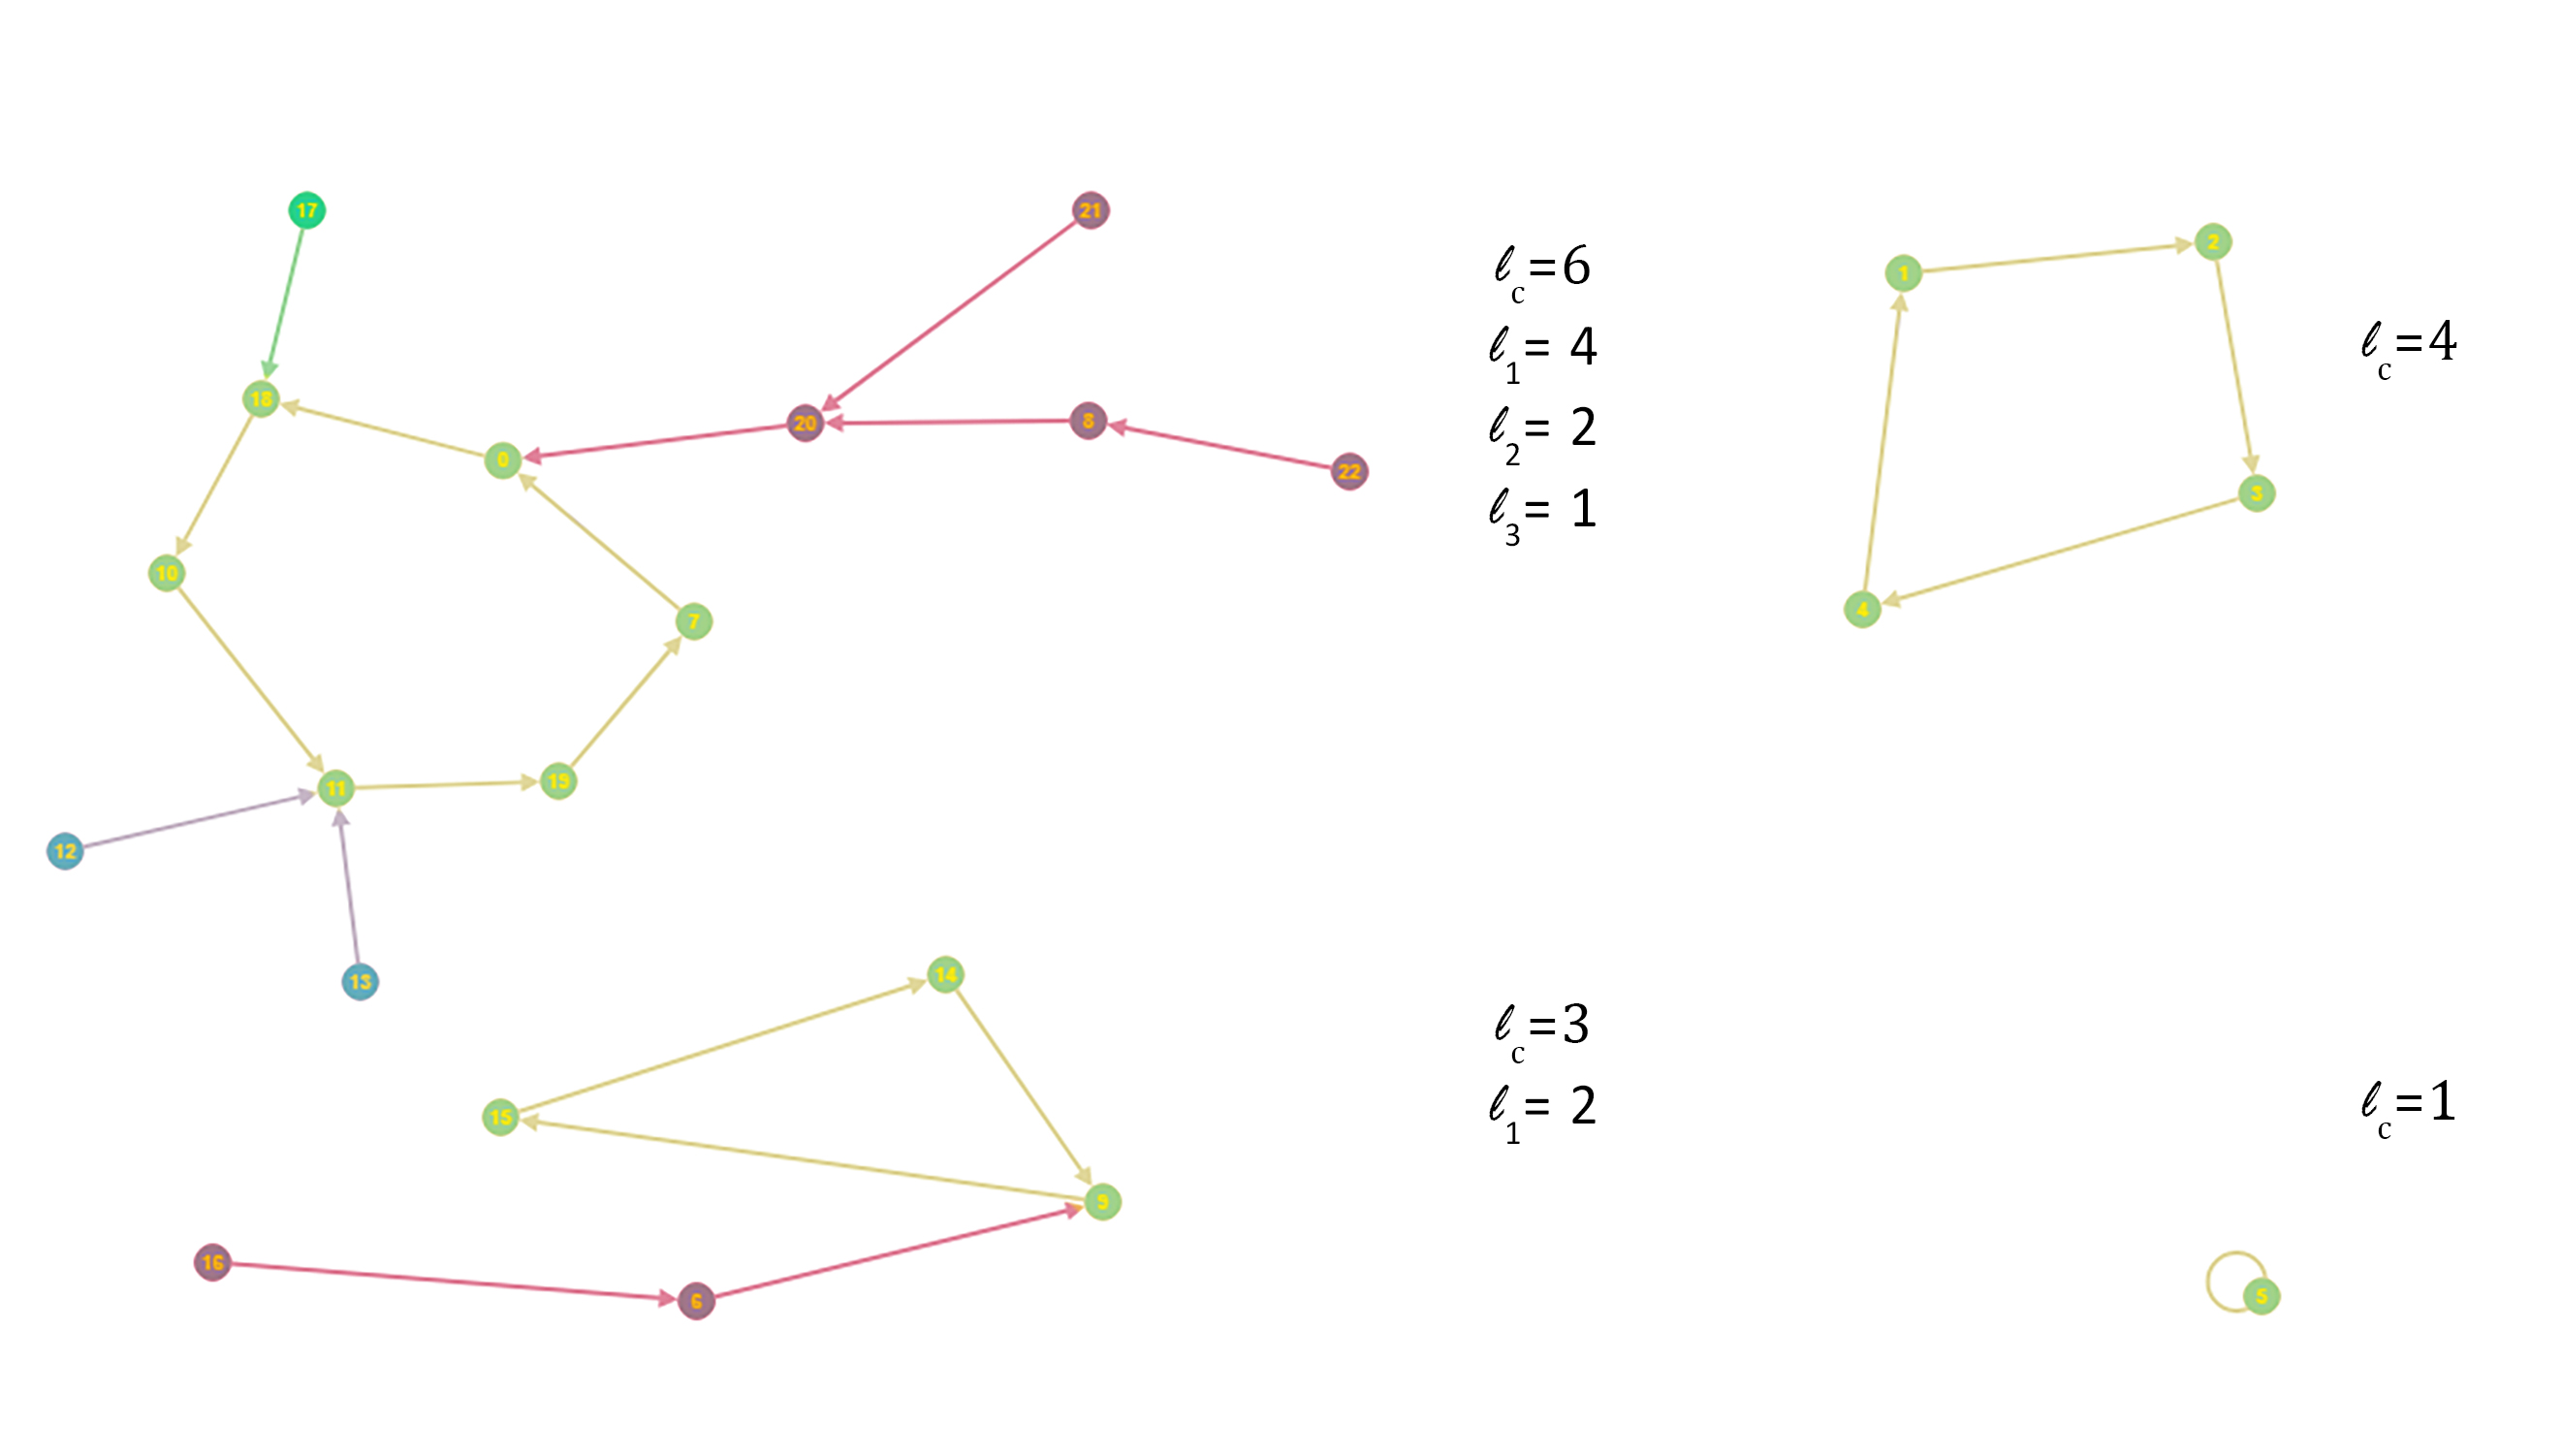
\includegraphics[width=0.75\textwidth]{graph_ex.jpg}
	\caption{Пример графа случайного отображения}
	\label{graph_ex}
\end{figure}

Очевидно, что в результате этого будет образовываться некоторое подобие леса. Каждая компонента в том графе будет ориентированным графом ровно с одним циклом, причем все ребра направлены в сторону этого цикла.

Теперь давайте приступим к количеству таких графов. Для начала начнем с одной компоненты. Введем следующие параметры, которые могут определить данную компоненту и определим число компонент с данными параметрами.

\begin{enumerate}
\item $n$ -- кол-во вершин в компоненте
\item $l_c$ -- число вершин находящихся в циклической части одной компоненты графа (изменяется от 1 до n)
\item $l_1, l_2, ..., l_k$ -- число вершин находящихся в "побочных путях" ведущих до циклической части графа без единицы, каждая из них больше $0$ и при этом в сумме они дают $n-l_c$. Стоит заметить, что под побочными путями имеются в виду ориентированные деревья, каждая из вершин которых имеет однозначный путь до цикла (в силу того, что это деревья)
\item $k$ -- число побочных путей" в графе.
\end{enumerate}
Для наглядности на рисунке \ref{graph_ex} желтым цветом определен цикл, другими цветами определены побочные компоненты и указаны соответствующие параметры графа.


Приступим к подсчетам.

Для первого "побочного пути" нужно выбрать какие вершины  будут в нем состоять ($\frac{n!}{l_1!(n - l_1)!}$ способов) После этого нужно будет разместить их на дереве, которое будет соединено в последствии с циклом. Согласно теоремы Келли о числе деревьев, число таких деревьев составляет $l_1^{l_1-2}$. После этого на этом дереве нужно будет выбрать вершину, которая будет соединена с циклом ($l_1$ способов) и непосредственно саму вершину на цикле, которая будет с ней соединена ($l_c$ способов). Очевидно, что выбирая соединительную вершину на дереве мы всегда однозначным образом определим направление, в котором будут идти стрелки от каждой другой вершины до соединительной(т.к. в дереве, кротчайший путь от одной вершины к другой всегда однозначен и в нем отсутствуют циклы). Итого получим кол-во способов получить искомую вершину:
$$\frac{n!}{l_1!(n- l_1)!}l_c l_1^{l_1-1}$$


То же самое проделываем для второго побочного пути, получим кол-во возможных комбинаций в этом случае  
$$\frac{(n- l_1)!}{l_2!(n- l_1 - l_2)!}l_c l_2^{l_2-1}$$


 и т.д. для $k$ой компоненты получим кол-во способов
$$
\frac{(n - l_1 - ... -l_{k-1})!}{l_k!(n - l_1 - l_2 - ... - l_k)!}l_c l_k^{l_k-1}=
\frac{(n - l_1 - ... -l_{k-1})!}{l_k!l_c!}l_c l_k^{l_k-1}
$$

Осталось выбрать только как будут расположены вершины на цикле ($(l_c-1)!$ способов. Мы убрали отсюда $l_c$ т.к. любую из этих вершин можно считать начальной)

Перемножая полученные комбинаторные значения получаем итоговую формулу

$$
\frac{n!}{(n - l_c)! l_c} \frac{(n- l_c)!}{l_1!(n - l_c - l_1)!}l_c l_1^{l_1-1} * ... * \frac{(n - l_c - l_1 - ... -l_{k-1})!}{l_k!(n - l_c - l_1 - l_2 - ... - l_k)!} l_c l_k^{l_k-1}=
$$
$$
= \frac{n!l_c^{k-1}l_1^{l_1-1}l_2^{l_2-1}...l_k^{l_k-1}}{l_1!l_2!...l_k!}=
C^{l_1, l_2, ..., l_k}_n l_c! l_c^{k-1}l_1^{l_1-1}l_2^{l_2-1}...l_k^{l_k-1}
$$
, где $C^{l_1, l_2, ..., l_k}_n$ -- мультиномиальный коэффициент,

Теперь нужно просуммировать данные значения при различных $l_1, l_2, ..., l_k$ и учитывая тот факт, что могут возникать повторения в результате такого подсчета связанные с выбором, какая компонента попадет в какой из побочных путей ($k!$ повторений) получаем итоговую формулу для подсчета количества числа таких компонент.

$$
\sum_{l_c=1}^n \sum_{k=0}^{n-l_c}\frac 1 {k!}\sum_{l_1+l_2+...+l_k=n-l_c} C^{l_1, l_2, ..., l_k}_n l_c! l_c^{k-1}l_1^{l_1-1}l_2^{l_2-1}...l_k^{l_k-1}=
$$
$$
\sum_{l_c=1}^n \frac {n!}{(n-l_c)!} \sum_{k=0}^{n-l_c} l_c^{k-1} \frac 1 {k!}\sum_{l_1+l_2+...+l_k=n-l_c} C^{l_1, l_2, ..., l_k}_{n-l_c} l_1^{l_1-1}l_2^{l_2-1}...l_k^{l_k-1}=
$$
Полученные числа, показывают кол-во компонент графа определенных выше(один цикл и все побочные компоненты ведут к нему), которые можно построить на $n$ вершинах. Обозначим их $M(n)$.


Стоит заметить, что данные числа встречаются в работе Дональда Кнута "Искуство программирования". В онлайн энциклопедии целочисленных последовательностей они занесены под номером A001865 и обозначают количество функций, у которых соответствующий им граф отображения имеет одну компоненту связанности (Number of connected functions on n labeled nodes).
В этой же энциклопедии имеется более простая формула для вычисления этих последовательностей

\begin{equation}
	\label{M-coef}
	\sum_{k=1}^n \frac{n!n^{n-k-1}}{(n-k!)}
\end{equation}

Причем $k$ое слагаемое внутри суммы это количество искомых графов, которые имеют цикл длины $k$

Зная данный факт, давайте попробуем найти экспоненциальную производящую функцию для данных чисел, т.к. если мы найдем ее, то вычисление данных чисел будет занимать всего одну строчку кода в языке Wolfram Mathematica и к тому же этот подсчет будет происходить гораздо быстрее. Для этого мы рассмотрим ряд вот такой функции.

$$-\ln(1+W(-x))$$
, где $W(x)$ --W функции Ламберта

Покажем, что именно она является экспоненциальной производящей для наших чисел. Начнем с ряда Тейлора W функции Ламберта.

$$
W(x) = \sum_{n=0}^{\infty} (-1)^{n-1}\frac{n^{n-1}x^n}{n!}
$$ 

Зная замечательное свойство ряда Тейлора для степени W-функции Ламберта, а именно:

$$
W^k(x) = -k \sum_{n=k}^\infty \frac{(-n)^{n-k-1}}{(n-k)!}x^n
$$ 
заметим, что данная формула очень напоминает слагаемые из формулы, которую мы нашли в онлайн энциклопедии для наших чисел. А именно, если мы рассмотрим такую функцию:

\begin{equation}
\label{cycle-coef}
(-1)^{k} \frac{W^k(-x)}{k} =  \sum_{n=k}^\infty \frac{n^{n-k-1}}{(n-k)!}x^n
\end{equation} , то заметим, что именно она будет являться экспоненциальной производящей функцией для количество односвязанных искомых графов, которые имеют цикл длины $k$

Теперь, если мы рассмотрим ряд Тейлора от функции:

$$
- W(-x) + \frac{W^2(-x)}{2} - \frac{W^3(-x)}{3} + \frac{W^4(-x)}{4} - ... =
$$ , то коэффициент при $x^n$ будет в точности как из формулы \eqref{M-coef}. Заметим, что такой ряд имеет именно функция 

$$
-\log(1+W(-x))
$$


Осталось только определить число графов, состоящих из таких компонент построенных на $n$ вершинах. 
Если в каждой компоненте будет $n_i$ вершин, а всего компонент $k$, то искомое число таких графов

\begin{equation}
\label{useless-coef}
\frac 1 {k!} \sum_{n_1+n_2+...+n_k=n} C^{n_1, n_2, ..., n_k}_n M(n_1)M(n_2)...M(n_k)
\end{equation}

Теперь, давайте попробуем найти экспоненциальную производящую функцию и для этих чисел. Покажем, что данные числа образованы производящей функцией

\begin{equation}
\label{W-coef}
(-1)^k \frac 1 {k!} \ln^k(1+W(-x))
\end{equation}

Действительно, если мы будем возводить наш ряд в степень $k$, то перед $x^n$ будет стоять именно число, стоящее в формуле 

Стоит отметить, что в вышеуказанной базе данных существует описание способа, описывающий как подсчитать количество функции, соответствующие графы которых обладают одной, двумя и тремя компонентами связанности. Все они основаны на W функции Ламберта, а точнее на ее коэффициентах в разложении в ряд Тейлора. 
Так например количество отображений над алфавитом мощности n с соответствующим графом обладающим 1ой компонентой связанности равно n-ому коэффициенту в формуле \eqref{useless-coef} под знаком суммирования (в силу особенностей возведения рядов в степень)

Данная особенность получения чисел с помощью экспоненциальной производящей функции позволит нам упростить расчеты, сделать их более эффективными в плане вычислений. Так на компьютере автора поиск искомых чисел с помощью формулы \eqref{useless-coef} позволял работать только с алфавитом мощности 20-30, в то время как работа с помощью формулы \eqref{W-coef} позволила добиться увеличения производительности в десятки раз.

Теперь приступим к подсчету чисел, ради которых и была написана данная глава этой работы, а именно подсчету суммарного числа компонент всех графов отображений. Зная суммарное число компонент можно без особых трудностей получить среднее число компонент поделив суммарное число компонент на количество всех функций ($n^n$).

Поскольку мы знаем, как получить число наших графов с $n$ вершинами обладающих $k$ компонентами (воспользовавшись тем фактом, что это $n$ый коэффициент в ряду Тейлора у функции \eqref{W-coef}), попробуем узнать вид экспоненциальной производящей функции коэффициенты ряда Тейлора которого -- суммарное число компонент всех графов соответствующие всем эндоморфизмам над множеством мощности n.

Если мы знаем кол-во графов с одной компонентой, двумя, тремя и т.д., то суммарное число компонент, это сумма произведений числа графов с k компонентами умноженными на k, где $k=1,...,n$.

т.к. эти числа лежат в коэффициентах функций вида \eqref{W-coef}, то проделаем данные манипуляции с этими функциями

$$\sum_{k=1}^{n} k (-1)^k \frac 1 {k!} \ln^k(1+W(-x))= 
\sum_{k=1}^{n} \frac 1 {(k-1)!} (-\ln(1+W(-x)))^k
$$

Заметим, что свободный коэффициент в \eqref{W-coef} всегда равен 0 (число отображений в графе с $n=0$ вершинами на $k\ne0$ компонентами равно 0). Поэтому с увеличением мощности алфавита и при произведении расчетов для эндоморфизмов над алфавитом мощности $n$, первые $k<n$ компонент будут такими же как и для расчетов для эндоморфизмов над алфавитом мощности $k$ т.к. в нашей формуле появится только $-\ln(1+W(-x))$ в степени $n$, а значит первые $k<n$ коэффициентов не изменятся.

Таким образом мы можем сделать переход до $n=\inf$ и брать оттуда нужные нам коэффициенты.  

$$
\sum_{k=1}^{\infty} \frac 1 {(k-1)!} p^k=
e^p*p
$$

Делая обратно подстановку $p=-\ln(1+W(-x))$ Получим

$$
\frac {-\ln(1+W(-x))}{(1+W(-x))}
$$

Таким образом, для того, чтобы получать среднее количество компонент графов функций над алфавитом мощности $n$ нужно взять $n$ый член ряда Тейлора полученной функции и поделить его на общее число функций ($n^n$). Как уже отмечалось выше, сам $n$ый коэффициент означает суммарное число компонент графа от всех отображений над алфавитом мощности $n$.

\section{Случай биективного случайного отображения}

Формула, полученная выше, решает задачу для случая любой функции (не обязательно биективной). В связи с тем, что автор находит весьма красивым формулу для числа суммарного числа компонент графов биективынх отображений, мы рассмотрим этот случай отдельно от функций общего вида.

В первую очередь заметим, что если мы будем рассматривать случай биективной функции, то графы, которые будут образовываться будут представлять циклы.

Выведем формулу для подсчета кол-ва способов получить из множества k различных непересекающихся циклов. Данная задача уже будет выглядеть довольно простой в сравнении с предыдущей задачей связанной с любой функцией. 

Рассмотрим случай, когда мы разбили наше множество на $k$ циклов длины $l_1, l_2, ..., l_k$. 

Стоит заметить что данные числа являются числами Стирлинга первого рода без знака и для них существует простая рекуррентная формула для подсчета.
Данная "особенность" не является случайной. Если внимательно посмотреть на определение чисел Стирлинга первого рода, то можно понять, что это именно те числа, которые мы и хотели получить изначально. А именно это количество перестановок из n элементов с k циклами.

Для вычисления данных чисел существует рекуррентное соотношение 


$$S(n, k) = S(n-1, k-1) + (n-1) S(n-1,k)$$
$$S(0,0) = 1$$
$$S(n,0) = 0, \text{ при } n>0$$
$$S(0,k) = 0, \text{ при } k>0$$

Смысл этого рекуррентного соотношения следующий. Для разбиения множества из $n$ элементов на $k$ циклов, можно взять уже готовое разбиение множества с $n-1$ элементами на $k-1$ циклов и добавить новый элемент в качестве нового цикл или же можно было взять разбиение множества c $n-1$ элементами на $k$ циклов и добавить новый элемент в один из готовых циклов ($n-1$ способ). 

Теперь приступим к подсчету среднего количества компонент графа. Обозначим через $A(n)$ среднее количество компонент графа для языка мощности $n$ при биективном отображении

$$A(n) = \frac 1 {n!}(1*S(n,1)+2*S(n,2)+...+n*S(n,n))=$$
$$\frac 1 {n!} (1*(S(n-1,1-1)+(n-1)*S(n-1,1))+2*((S(n-1,2-1)+(n-1)*S(n-1,2)))+...+n*((S(n-1,n-1)+(n-1)*S(n-1,n))))=$$
$$\frac 1 {n!} (1*((n-1)*S(n-1,1))+2*((S(n-1,2-1)+(n-1)*S(n-1,2)))+...+n*((S(n-1,n-1))))=$$
$$\frac 1 {n!} ((n-1)*(1*S(n-1,1)+2*S(n-1,2)+...+(n-1)*S(n-1,n-1)) + 2*S(n-1,1)+3*S(n-1,2)+...+n*S(n-1,n-1))=$$
$$\frac 1 {n!} (n*(1*S(n-1,1)+2*S(n-1,2)+...+(n-1)*S(n-1,n-1)) + S(n-1,1)+S(n-1,2)+...+S(n-1,n-1))=$$
$$\frac 1 {n!} (n*A(n-1) + (n-1)!)=$$

Очевидно, что $A(1)=1$.
Теперь от рекурсивной функции перейдем к непосредственной 

$$A(n) = \frac 1 {n!} (n*A(n-1) + (n-1)!) = \frac 1 {n!} (n*((n-1)A(n-2)+(n-2)!) + (n-1)!)=$$
$$\frac 1 {n!} (n*((n-1)((n-2)A(n-3)+(n-3)!)+(n-2)!) + (n-1)!)=$$
$$\frac 1 {n!} (n*((n-1)((n-2)A(n-3)+(n-3)!)+(n-2)!) + (n-1)!)=$$
$$\frac 1 {n!} (n*((n-1)((n-2)(...3(2*1+1!)+2!)...+(n-3)!)+(n-2)!) + (n-1)!)=$$
$$\frac 1 {n!} (n!+\frac{n!}{2}+\frac{n!}{3}+...+\frac{n!}{n-1}+\frac{n!}{n})=$$
$$ 1+\frac{1}{2}+\frac{1}{3}+...+\frac{1}{n-1}+\frac{1}{n}= \sum_{k=1}^n \frac 1 k$$

То есть среднее количество компонент графа, относящемуся к биективному отображению над алфавитом мощности $n$ на себя, является $n$ым гармоническим числом.
Этот факт показывает например, что с увеличением мощности алфавита число компонент стремится к бесконечности (из свойств гармонических чисел).

\section{Анализ полученных формул}


\mychapter{3}{Оценка числа компонент графа итерации случайного отображения}

\section{Основная часть}

Перейдем теперь к сути исходной задачи, которая стояла  перед нами, а именно как будет изменяться суммарное число компонент графа при итерации случайного отображения.

В первую очередь заметим, что при итерации отображения мы будем перепрыгивать через несколько ребер нашего графа, причем в результате данного "перепрыгивания" циклы могут распадаться и собираться вместе. Из этого свойства следует один из важных фактов, который позволит вычислить нам при какой степени суммарное число компонент графа будет максимальным. А именно, давайте рассмотрим при каком условии наши компоненты содержащие циклы распадутся на компоненты содержащие циклы длины 1. Такое возможно если в каждом цикле, любой длины мы будем возвращаться обратно в своб же вершину. Для этого нужно, чтобы степень отображения делилась на длину любого цикла в компонентах, то есть была наименьшим общим кратным для всех чисел начиная с единицы и заканчивая длиной самого максимального цикла (то есть мощности алфавита). То есть, например, для 5 это число будет $\lcm(1,2,3,4,5) = 60$. 

Данный фаbкт мы оставим на рассмотрение в следующем разделе, а теперь перейдем к основной задаче. Начнем с того, что узнаем на сколько компонент распадется одна компонента графа при возведении случайного отображения в степень $r$. Если данная компонента имеет цикл длины $k$, то число компонент, на которое распадется данная компонента при возведении отображения в степень $r$ будет $\gcd(r,k)$.Докажем данный фат

\begin{proof}
	
	Пусть $n$ -- минимальное число вершин, которые мы пройдем до тех пор, пока не попадем в исходную, которая стоит на позиции $p$. Тогда, должно выполнится равенство
	
	$p=p+r n\mod k$
	
	Поскольку $n$ является минимальным, то оно должно ровняться $k/\gcd(r,k)$. Действительно, пусть $z$ -- это минимальное число, при котором выполняется данное равенство. Заметим, что наше условие эквивалентно условию
	
	$r z = 0\mod k$, а значит в силу свойств сравнения по модулю должно выполняться и то, что 
	
	$\alpha_1 z = 0 \mod \alpha_2$, где $\alpha_1= \frac r {\gcd(r,k)}$, а $\alpha_2= \frac k {\gcd(r,k)}$. В силу того, что $\alpha_1$ и $\alpha_2$ взаимопросты, то данное равенство выполняется только при $z=\alpha_2$, что мы и хотели показать. А следовательно и число циклов, на которое распадется компонента будет $\gcd(r,k)$. Т.к. при прохождении всех вершин, начиная с какой-либо, мы разбиваем наш цикл на непересекающиеся циклы длины $\frac k {\gcd(r,k)}$, скольких у нас ${\gcd(r,k)}$
\end{proof}	

На "побочные" можно не обращать внимания т.к. они не смогут создать новый цикл (в силу их ацикличности) и соединятся с одним из образовавшихся циклов. Так же стоит заметить, что в результате итерации отображения, две компоненты слиться не смогут в силу того, что одна компонента не имеет общих вершин с другой из вершины лежащей на одной компоненте, за любое число шагов, не возможен до вершины другой компоненты

Теперь, когда мы знаем на сколько компонент распадется наша компонента, которая обладает циклом длины $k$, то мы можем найти производящую функцию для суммарного числа компонент при возведении отображений, граф которых обладает всего одной компонентой, в степень. 

Как мы помним из прошлой главы функция \eqref{cycle-coef} является экспоненциальной производящей для числа связанных графов, которые обладают циклом длины $k$. Значит экспоненциальная производящая функция для суммарного числа компонент которые образуются при возведении отображения в степень,граф которых обладает циклом длины $k$, будет:

$$\gcd(r,k) (-1)^{k} \frac{W^k(-x)}{k}$$

Докажем свойство наибольшего общего делителя, которое понадобится нам в дальнейшем, заключающееся в том, что $\gcd(m,n)=\gcd(m+i*n,n)$ при любых целых $i$

\begin{proof}
	Пусть $d=\gcd(m,n)$, тогда$d a_1=m, d a_2 = n$, используя тот факт из теории чисел заключающийся в том, что существуют такие числа $b_1, b_2$, такие что
	
	$$m*b_1+n*b_2 = d$$ причем $d$ -- минимальное положительное значение функции стоящей слева при целых $b_1$ и $b_2$
	
	представим $b_2$ как $i b_1+b_2'$, получим
	
	$$b_1*(m+ i n) + b_2'*n=d$$, в силу того, что меньше значение у этой функции получиться не может (иначе было получилось меньше значение у функции выше), то это и есть наибольший общий делитель чисел $m+i n$ и $n$
	
\end{proof}

Зная данный факт, мы можем сказать, что число компонент, на которое распадется компонента с циклом длины $k$ совпадает с числом компонент на которое распадется компонента с циклом длины $k+i r$. Теперь, можно приступить к подсчету суммарного числа компонент графов, которые имеют одну компоненту, в результате его распада при возведении в степень.

Т.к. число компонент, которые имеют циклы длины $k$ равно $(-1)^{k} \frac{W^k(-x)}{k}$, то производящая функция для тех чисел, которые мы хотим найти будет

$$
-\gcd(r,1) W(-x) + \gcd(r,2) \frac{W^2(-x)}{2} - \gcd(3,k) \frac{W^3(-x)}{3} + ... +$$
$$
+\gcd(r,r-1) (-1)^{r-1} \frac{W^{r-1}(-x)}{r-1} + \gcd(r,r) (-1)^{r} \frac{W^r(-x)}{r} + \gcd(r,1) (-1)^{r+1} \frac{W^{r+1}(-x)}{r+1} + ... +
$$
$$
+\gcd(r,r-1) (-1)^{2r-1} \frac{W^{2r-1}(-x)}{2r-1} + \gcd(r,r) (-1)^{2r} \frac{W^{2r}(-x)}{2r} + \gcd(r,1) (-1)^{2r+1} \frac{W^{2r+1}(-x)}{2r+1} + ... +
$$
$$
...
$$
$$
=
$$
$$
-\gcd(r,1)(W(-x) + (-1)^{r} \frac{W^{r+1}(-x)}{r+1} + (-1)^{2r} \frac{W^{2r+1}(-x)}{2r+1} +  ...)+ 
$$
$$
+\gcd(r,2)(\frac{W^2(-x)}{2} + (-1)^{r} \frac{W^{r+2}(-x)}{r+2} + (-1)^{2r+2} \frac{W^{2r+2}(-x)}{2r+2} +  ...)+ ... +
$$
$$
+(-1)^r\gcd(r,r)(\frac{W^r(-x)}{r} + (-1)^{r} \frac{W^{2r}(-x)}{2r} + (-1)^{3r} \frac{W^{3r}(-x)}{3r} +  ...)
$$

Посмотрим, чему равен ряд находящийся внутри скобок. Он имеет вид:

$$
\sum_{n=0}^{\infty} (-1)^{n r}\frac {x^{n r+k}}{n r+k}
$$

Для того, чтобы узнать, чему равен этот ряд рассмотрим гипергеометрическую функцию $_2F_1(a,b,c,x)$, ряд которой имеет вид:

$$
_2F_1(a,b,c,x) = \sum_{n=0}^{\infty}\frac{(a)_n(b)_n}{(c)_n} \frac {x^n}{n!}
$$, где $(x)_n$ символ Похгаммера
$$(x)_n = \prod_{k=1}^{n} (x+k-1)= x(x+1)(x+2)...(x+n-1)$$

Тогда можно заметить, что если мы рассмотрим ряд функции $_2F_1(1, \frac k r, \frac k r +1, (-x)^r) \frac {x^k} k$, то ее ряд будет иметь нужный нам вид. Действительно.

$$
_2F_1(1, \frac k r, \frac {k+r} r, (-x)^r) = \sum_{n=0}^{\infty} \frac{n!(\frac k r)(\frac k r +1)...(\frac k r +n-1)}{(\frac k r +1)...(\frac k r +n)} \frac{(-1)^{nr} x^{nr}}{n!}= \sum_{n=0}^{\infty} \frac{\frac k r}{\frac k r +n} (-1)^{nr} x^{nr} = \sum_{n=0}^{\infty} \frac{k}{n r+k} (-1)^{nr} x^{nr}
$$

Таким образом, если мы домножим получившийся ряд на $\frac {x^k} k$, то мы получим искомый ряд. Следовательно искомая экспоненциальная производящая функция имеет вид

\begin{eqnarray}
\label{main-coef}
\sum_{k=1}^r (-W(-x))^k \gcd(r,k) \frac {_2F_1(1, \frac k r, \frac k r +1, (-(W(-x)))^r)} k 
\end{eqnarray}

Обозначим данную функцию как $F(r,x)$. Нетрудно заметить, что формула полученная ниже, для одной степеня $r=1$ является частным случаем полученной формулы.

Теперь осталось узнать производящую функцию суммарного числа компонент образующихся в результате возведения всех отображений в степень $r$. Поскольку отображение состоит из нескольких компонент (обозначим это число как $a$) и каждая компонента состоящая из $k$ вершин образует в результате число компонент равное $k$ому коэффициенту $F(r,x)$ (обозначим это число как $b$). Таким образом число раз, в которое увеличилось число компонент равняется $\frac {b}{a}$

Теперь, пусть отображение состоит из компонент мощности $n_1, n_2, ..., n_k$ (некоторые из них могут быть равны 0) и существует всего $a_{n_i}$ компонент над алфавитом мощности $n_i$, где $i=1,2...,k$. Тогда первая компонента увеличится в $\frac {b_{n_1}} {a_{n_1}}$ раз, вторая в $\frac {b_{n_2}} {a_{n_2}}$ раз и т.д. $k$ая компонента увеличится в $\frac {b_{n_k}} {a_{n_k}}$ раз. Т.к. число всех таких отображений будет $C_n^{n_1,n_2,...,n_k}a_{n_1}a_{n_2}...a_{n_k}$. Таким образом суммарное число компонент которое образуется в результате определенных $a_{n_1},a_{n_2},...,a_{n_k}$ будет

$$
C_n^{n_1,n_2,...,n_k}(\frac {b_{n_1}} {a_{n_1}}+ \frac {b_{n_2}} {a_{n_2}} + ... + \frac {b_{n_k}} {a_{n_k}})a_{n_1}a_{n_2}...a_{n_k}
$$, что равносильно 

$$
C_n^{n_1,n_2,...,n_k}\sum_{i=1}^{k} b_{n_i} a_{n_1} a_{n_2}...a_{n_{i-1}}a_{n_{i+1}}...a_{n_k}
$$

Просуммируем по всевозможным $n_1, n_2, ..., n_k$ и поделим на число повторений $k!$

$$
\frac 1 {k!}\sum_{n_1+...+n_k=n}C_n^{n_1,n_2,...,n_k}\sum_{i=1}^{k} b_{n_i} a_{n_1} a_{n_2}...a_{n_{i-1}}a_{n_{i+1}}...a_{n_k}
$$

Т.к. $a_i$ это $i$ый коэффициент у $F(1,x)$, а $b_i$ это $iый$ коэффициент у $F(r,x)$, где $i=1,2,...,k$.

Тогда нетрудно убедиться, что производящая функция для отображения с $k$ числом компонент будет 

$$\frac 1 {(k-1)!} F(r,x)F^{k-1}(1,x)$$

Так будет получаться в силу свойств перемножения рядов и при коэффициенте $x^n$ будет именно нужный нам коэффициент. Действительно:

$$
\frac 1 {(k-1)!} F(r,x)F^{k-1}(1,x) = \frac 1 {(k-1)!}  \sum_{n_1=0}^{\infty} \frac{b_{n_1}}{n_1!} x^{n_1}\sum_{n-n_1=0}^\infty\left(\sum_{n_2+...+n_k=n-n_1} C_{n-n_1}^{n_2,...,n_k} a_{n_2}...a_{n_k}\right)\frac {x^{n-n_1}}{(n-n_1)!}=
$$
$$
\frac 1 {(k-1)!}  \sum_{n=0}^\infty\left(\sum_{n_1+n_2+...+n_k=n} C_{n}^{n_1, n_2,...,n_k} b_{n_1}a_{n_2}...a_{n_k}\right)\frac {x^n}{n!}=
$$
$$
 \sum_{n=0}^\infty \left( \frac 1 {k!} \sum_{n_1+n_2+...+n_k=n} C_{n}^{n_1, n_2,...,n_k} \sum_{i=1}^{k}b_{n_i} a_{n_1} a_{n_2}...a_{n_{i-1}}a_{n_{i+1}}...a_{n_k}\right)\frac {x^n}{n!}
$$

Что и требовалось показать.

На финальном шаге нам осталось просуммировать это число при всевозможных $k$, так же как и в случае с $r=1$. Производя такое суммирование получим:

$$\sum_{k=1}^{\infty}\frac 1 {(k-1)!} F(r,x)F^{k-1}(1,x) = F(r,x)e^{F(1,x)}$$

На этом этапе вспоминаем, что 

$$
F(1,x) = -\log(1+W(-x))
$$

И таким образом получаем итоговую формулу:

$$
\frac{F(r,x)}{1+W(-x)}
$$, где F(r,x) -- это функция \eqref{main-coef}

Данная экспоненциальная производящая функция позволяет легко определить суммарное количество компонент, которое образуется в результате итерации случайного отображения. Если же мы хотим определить наиболее вероятное число компонент, которое мы получим, в результате применения случайного отображения, то надо поделить это число на число отображений ($n^n$). 

Как это не странно, формула полученная в первой главе является всего лишь частным случаем полученной формулы в этой главе. Более того, получив экспоненциальную производящую функцию для наших чисел, мы опять-таки облегчили программирование нашей формулы (на языке Wolfram Mathematica расчеты производятся в 3 строчки. При желании (и потери читабельности кода) данную формулу можно записать и в одну строчку), увеличение производительности при расчете чисел. Так, для сравнения, при поиске данных чисел "в лоб" (т.е. грубым перебором всех отображений) поиск числа компонент затягивался на несколько минут для $r=2$ и мощности алфавита $n=6$, в то время, как при использовании производящей функции мы могли работать с алфавитом мощности $n=600$ и степенью $r=2$, при этом на все расчеты уходило примерно 45 секунд!

\section{Оценка числа максимального числа компонент при итерации случайного отображения}

В данном разделе давайте попробуем найти каким будет суммарное максимального число компонент, которое будет получаться при итерации случайного отображения, то есть когда степень является $i (1,2,...,n)$ для отображений над алфавитом мощности $n$.

Насколько мы знаем из начала первого раздела данной главы, число компонент на которое распадется наша компонента с циклом длины $k$ будет $k$. Основываясь на этом факте и еще используя то же свойство, которое мы использовали в первой главе и основной части данной работы об экспоненциальной производящей функции числа компонент с циклом длины $k$ (то есть функции \eqref{cycle-coef}), мы можем найти производящую функцию для суммарного числа компонент, на которое распадется на которые будут распадаться всевозможные связанные компоненты графа построенного на $n$ вершинах. А именно:

$$
-W(-x) +  W^2(-x) - W^3(-x) + ... = \frac{1}{1+W(-x)} - 1 = \frac{-W(-x)}{1+W(-x)}
$$

Зная данный факт мы можем теперь с легкостью найти суммарное максимальное число компонент графа отображения, которое образуются в результате итерации отображения, граф которого имеет $k$ компонент, нужное количество раз. А именно, по аналогии с прошлыми разделами экспоненциальная производящая функция будет

$$
\frac 1 {(k-1)!} \frac{-W(-x)}{1+W(-x)} (-\log(1+W(-x)))^{k-1}
$$

В целях экономии места в данной статье оставим доказательства этого факта в качестве упражнения на усвоение материала читателю

Теперь так же, как и в остальных случаях просуммируем при всевозможных $k$, получим производящую функцию следующего вида:

$$
\sum_{k=1}^{\infty}\frac 1 {(k-1)!} \frac{-W(-x)}{1+W(-x)} (-\log(1+W(-x)))^{k-1}=
\frac{-W(-x)}{(1+W(-x))^2}
$$

Данный результат мы более подробно рассмотрим в последующих разделах, когда будем находить асимптотическую функцию коэффициентов данной экспоненциальной производящей функции.

\section{Оценка числа компонент итерации биективного случайного отображения}

Начнем поиск экспоненциальной производящей функции для данной задачи начиная с тех же соображений, которые мы использовали в начале первого раздела (т.е. мы будем отталкиваться от того, что мы знаем, на сколько распадется компонента с циклом длины $k$). 

Приступим сразу к подсчету числа компонент, которые образуются в результате итерации $r$ раз биективного случайного отображения с одной компонентой в графе

$$
\gcd(r,1)\frac{0!}{1!}x + \gcd(r,2)\frac{1!}{2!}x^2 + ... + \gcd(r,r-1)\frac{(r-2)!}{(r-1)!}x^{r-1} + \gcd(r,r)\frac{(r-1)!}{r!}x^r + \gcd(r,1)\frac{r!}{(r+1)!}x^{r+1} + ... = 
$$
$$
\gcd(r,1)(\frac {0!}{1!}x + \frac{r!}{(r+1)!}x^{r+1}+...)+ ... + \gcd(r,r)(\frac{(r-1)!}{r!}x^r+\frac{(2r-1)!}{(2r)!}x^{2r}+...)= 
$$
$$
\gcd(r,1)(\frac {1}{1}x + \frac{1}{r+1}x^{r+1}+...)+ ... + \gcd(r,r)(\frac{1}{r}x^r+\frac{1}{2r}x^{2r}+...)= 
$$

Если мы узнаем, какая функция имеет ряд вида

$$
\sum_{n=0}^{\infty}\frac{x^{n r + k}}{nr+k}
$$
, то  это позволит нам записать нашу функцию более компактно. К счастью, данная функция существует и называется дзета-функцией Гурвица и обозначается как $\Phi(x,s,\alpha)$. Ее ряд имеет вид:

$$
\Phi(x,s,\alpha) = \sum_{n=0}^{\infty}\frac{x^n}{(n+\alpha)^s}
$$

Нетрудно проверить, что в нашем случае мы имеем дело с функцией $x^k \Phi(x^r,1,\frac{k}{r})/r$

Теперь зная данный факт, мы можем записать нашу экспоненциальную производящую функцию более компактно, а именно:

$$
\sum_{k=1}^r \gcd(r,k) \frac{x^k \Phi(x^r,1,\frac{k}{r})}{r}
$$

Обозначим данную функцию как $F_b(r,x)$.

Т.к. производящая функция для числа биективных отображений с одной компонентой в графе это $-\log(1-x)$ (проверьте это!), то производящая функция для числа компонент, которые будут образовываться в результате итерации отображения, граф которого имеет $k$ компонент будет, по аналогии с прошлым разделом:

$$
\frac 1 {(k-1)!} F_b(z,x)(-\log(1-x))^{k-1}
$$

Проверьте данный факт, для закрепления материала!

Теперь опять-таки все суммируем по всевозможным $k$ и получаем экспоненциальную производящую функцию для суммарного числа компонент, а именно:

$$
\sum_{k=1}^{\infty}\frac 1 {(k-1)!} F_b(z,x)(-\log(1-x))^{k-1}= \frac{F_b(z,x)}{1-x}
$$

Мы опять-таки получили более общую формулу для подсчета числа компонент чем ту, что получили в первой главе. 

Заметим, что если мы хотим узнать вероятное число образовавшихся компонент в случае итерации случайно взятого отображения, то надо поделить число, которое мы получим, на общее число биективных отображений ($n!$)

Раздел посвященный подсчету максимального числа компонент, которые могут образоваться в результате итерации случайного отображения будет бессмысленным, т.к. число получившихся компонент будет очевидно -- $n$, для алфавита мощности n. Связанно это с тем, что все вершины будут находиться в циклах (в силу биективности) и все циклы распадутся на циклы длины $n$.


\mychapter{4}{Список используемой литературы}



\end{document}